% Story mode, proposed: where each part lives in the code. Solid boxes exist
% today; dashed boxes are new. The arrows follow data from the story file to
% the page, the same path the road takes (data -> content -> sim -> wasm -> page).
% Standalone: compiles with pdflatex.
\documentclass[tikz,border=4pt]{standalone}
\usetikzlibrary{arrows.meta,positioning,calc}

% --- Colors: the game's palette ------------------------------------------------
\definecolor{paper}{HTML}{EFE8D8}
\definecolor{ink}{HTML}{2B2A28}
\definecolor{muted}{HTML}{6B6457}
\definecolor{indigo}{HTML}{3E4A89}  % new work
\definecolor{ground}{HTML}{D9CDB2}  % existing work

% --- Layout -----------------------------------------------------------------------
\newcommand{\ColGap}{6.0}   % distance between columns, cm
\newcommand{\BoxW}{5.0cm}   % width of every box

\begin{document}
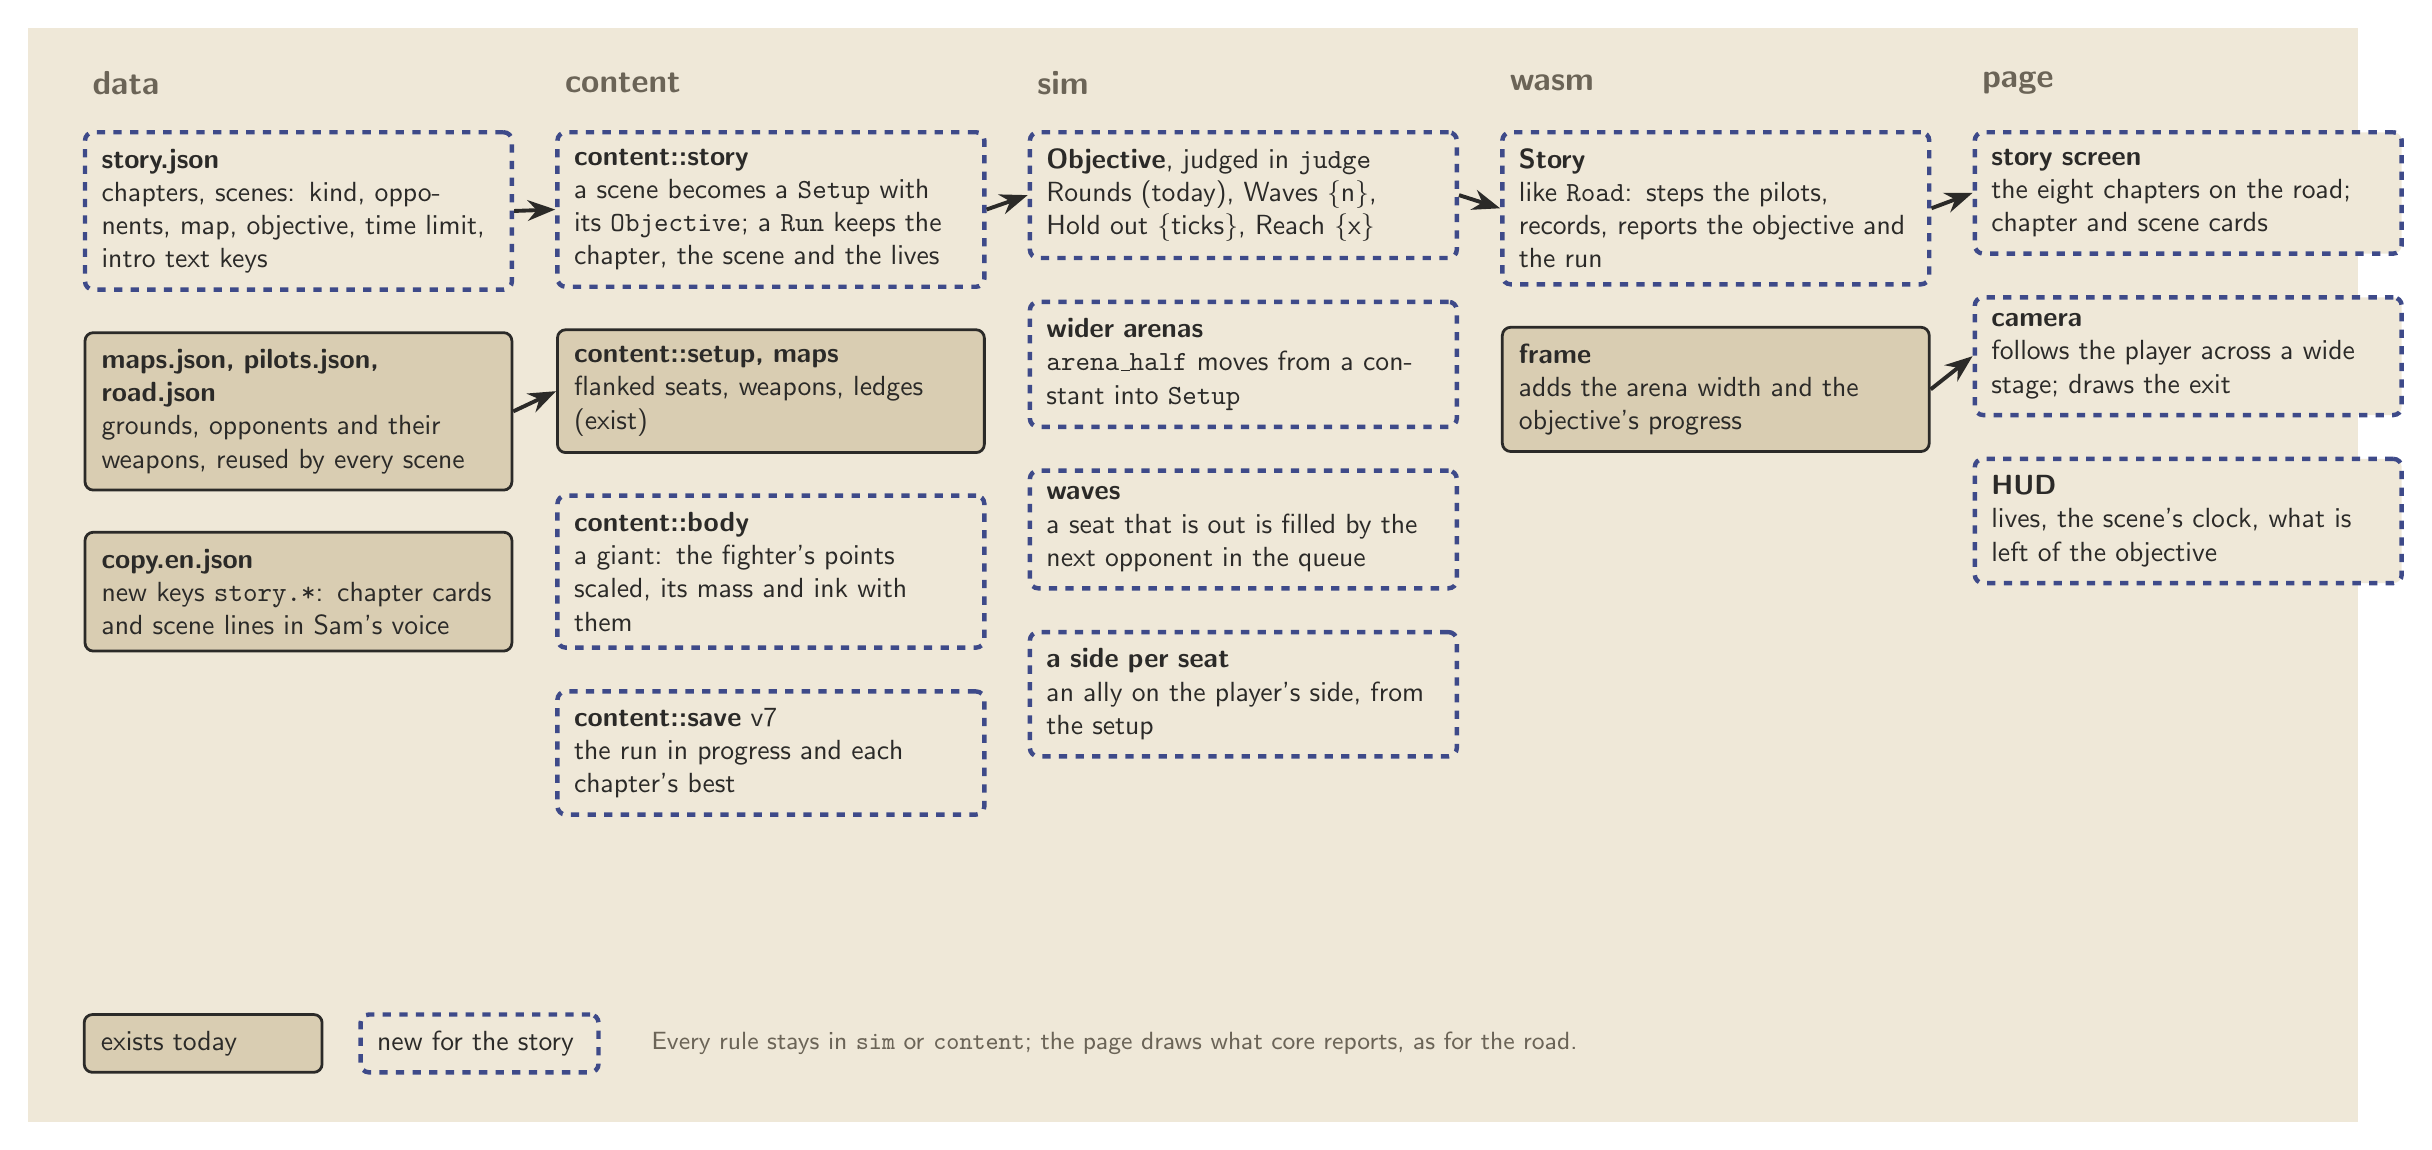
\begin{tikzpicture}[font=\sffamily, ink, node distance=0.5cm,
    old/.style={draw=ink, line width=1pt, fill=ground, text width=\BoxW, align=left, inner sep=6pt, rounded corners=3pt},
    new/.style={draw=indigo, dashed, line width=1.6pt, fill=paper, text width=\BoxW, align=left, inner sep=6pt, rounded corners=3pt},
    head/.style={font=\sffamily\bfseries\large, text=muted},
    flow/.style={-{Stealth[length=3.5mm]}, line width=1.4pt, draw=ink},
  ]
% --- Background --------------------------------------------------------------------
\fill[paper] (-1.0,1.3) rectangle (4*\ColGap+4.6,-12.6);

% --- Columns: data, content, sim, wasm, page --------------------------------------
\foreach \c/\h in {0/data,1/content,2/sim,3/wasm,4/page}
  \node[head, anchor=west] at (\c*\ColGap-0.3,0.6) {\h};

% data
\node[new, anchor=north west] (story) at (-0.3,0) {\textbf{story.json}\\chapters, scenes: kind, opponents, map, objective, time limit, intro text keys};
\node[old, below=of story] (maps) {\textbf{maps.json, pilots.json, road.json}\\grounds, opponents and their weapons, reused by every scene};
\node[old, below=of maps] (copy) {\textbf{copy.en.json}\\new keys \texttt{story.*}: chapter cards and scene lines in Sam's voice};

% content
\node[new, anchor=north west] (cstory) at (\ColGap-0.3,0) {\textbf{content::story}\\a scene becomes a \texttt{Setup} with its \texttt{Objective}; a \texttt{Run} keeps the chapter, the scene and the lives};
\node[old, below=of cstory] (setup) {\textbf{content::setup, maps}\\flanked seats, weapons, ledges (exist)};
\node[new, below=of setup] (body) {\textbf{content::body}\\a giant: the fighter's points scaled, its mass and ink with them};
\node[new, below=of body] (save) {\textbf{content::save} v7\\the run in progress and each chapter's best};

% sim
\node[new, anchor=north west] (obj) at (2*\ColGap-0.3,0) {\textbf{Objective}, judged in \texttt{judge}\\Rounds (today), Waves \{n\}, Hold out \{ticks\}, Reach \{x\}};
\node[new, below=of obj] (wide) {\textbf{wider arenas}\\\texttt{arena\_half} moves from a constant into \texttt{Setup}};
\node[new, below=of wide] (waves) {\textbf{waves}\\a seat that is out is filled by the next opponent in the queue};
\node[new, below=of waves] (team) {\textbf{a side per seat}\\an ally on the player's side, from the setup};

% wasm
\node[new, anchor=north west] (shim) at (3*\ColGap-0.3,0) {\textbf{Story}\\like \texttt{Road}: steps the pilots, records, reports the objective and the run};
\node[old, below=of shim] (frame) {\textbf{frame}\\adds the arena width and the objective's progress};

% page
\node[new, anchor=north west] (screen) at (4*\ColGap-0.3,0) {\textbf{story screen}\\the eight chapters on the road; chapter and scene cards};
\node[new, below=of screen] (camera) {\textbf{camera}\\follows the player across a wide stage; draws the exit};
\node[new, below=of camera] (hud) {\textbf{HUD}\\lives, the scene's clock, what is left of the objective};

% --- Flow (drawn last) ---------------------------------------------------------------
\draw[flow] (story.east) -- (cstory.west);
\draw[flow] (maps.east) -- (setup.west);
\draw[flow] (cstory.east) -- (obj.west);
\draw[flow] (obj.east) -- (shim.west);
\draw[flow] (shim.east) -- (screen.west);
\draw[flow] (frame.east) -- (camera.west);

% --- Legend ------------------------------------------------------------------------------
\node[old, text width=2.6cm, anchor=west] at (-0.3,-11.6) {exists today};
\node[new, text width=2.6cm, anchor=west] at (3.2,-11.6) {new for the story};
\node[anchor=west, text=muted, font=\sffamily\small, text width=17cm] at (6.8,-11.6)
  {Every rule stays in \texttt{sim} or \texttt{content}; the page draws what core reports, as for the road.};
\end{tikzpicture}
\end{document}
